\section{Pipeline Clássica: da Imagem ao Mapa de Ocupação}
\label{sec:metodologia}

A Figura~\ref{fig:pipeline-overview} resume as etapas descritas nesta seção: da imagem
bruta à obtenção de um mapa de ocupação e cor por casa. Todas as etapas usam apenas
técnicas clássicas de processamento de imagens.

\begin{figure}[H]
  \centering
  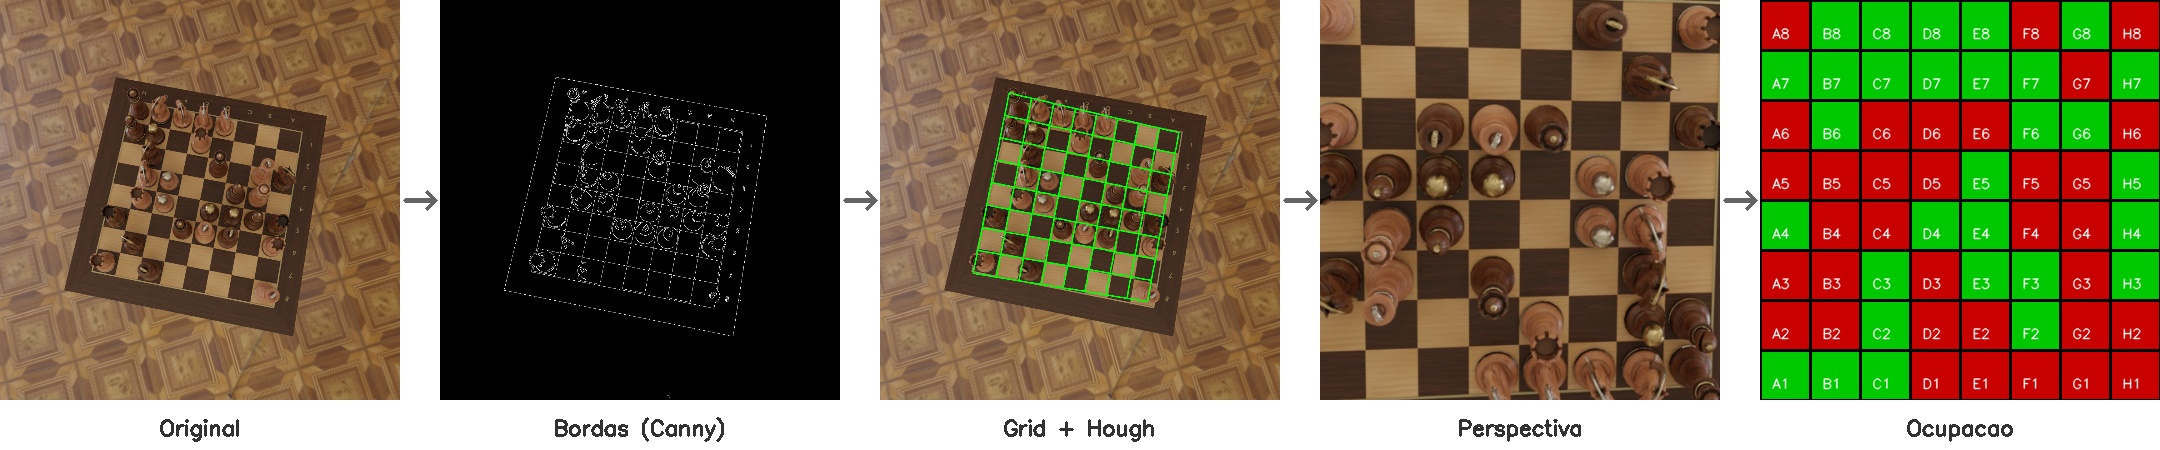
\includegraphics[width=0.85\textwidth]{../../intro/images/slide_pipeline.jpg}
  \caption{Visão geral da pipeline clássica: bordas, linhas de Hough, homografia,
    segmentação 8$\times$8, votação de características.}
  \label{fig:pipeline-overview}
\end{figure}

\subsection{Pré-processamento}

A imagem é convertida para tons de cinza usando a luminância perceptual do OpenCV
(\texttt{COLOR\_BGR2GRAY}), $Y = 0{,}114B + 0{,}587G + 0{,}299R$, pois a maioria dos
operadores de borda opera sobre imagens monocromáticas. Em seguida aplica-se suavização
gaussiana (kernel $5\times5$, $\sigma$ calculado automaticamente pelo OpenCV) para
reduzir ruído de alta frequência antes da detecção de bordas --- ruído gera gradientes
espúrios que se traduzem em bordas falsas.

Histograma de intensidade, equalização global (\texttt{equalizeHist}) e CLAHE
(\texttt{clipLimit=2.0}, \texttt{tileGridSize=(8,8)}) foram usados como ferramentas de
diagnóstico da distribuição de intensidade do dataset, mas não fazem parte da pipeline
principal.

\begin{figure}[H]
  \centering
  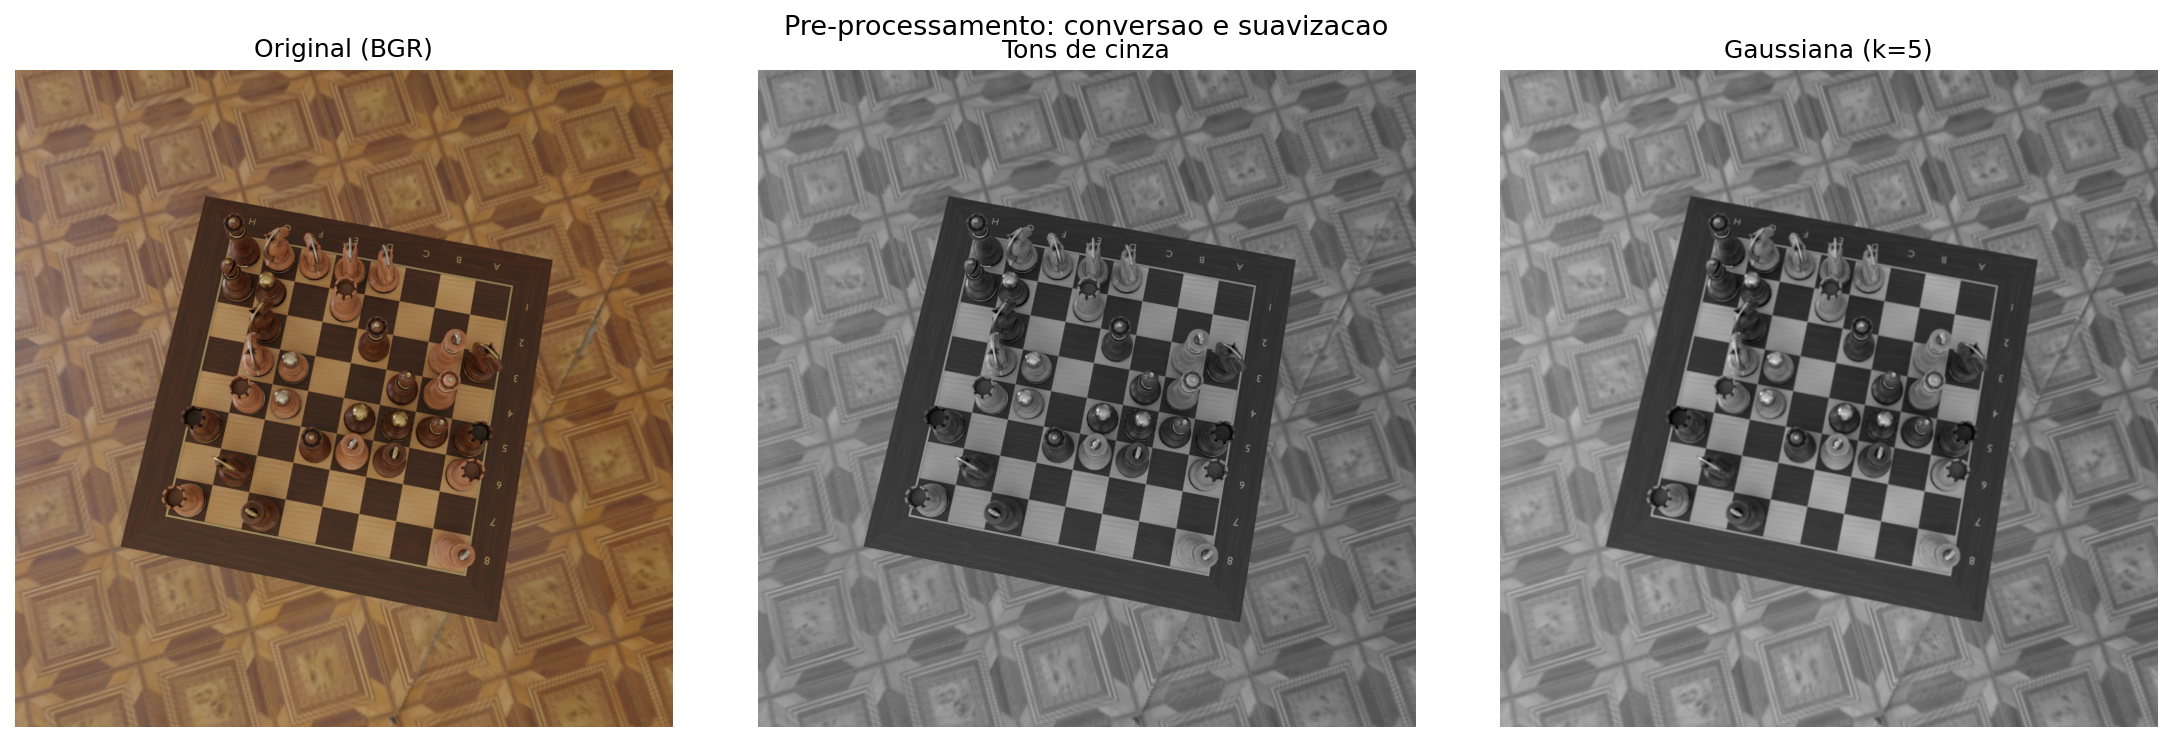
\includegraphics[width=0.75\textwidth]{../../intro/images/03_preprocessing.png}
  \caption{Conversão para tons de cinza e suavização gaussiana.}
\end{figure}

\subsection{Detecção de bordas}

Quatro operadores foram comparados: Roberts (kernel $2\times2$ cruzado, muito sensível a
ruído), Prewitt (kernel $3\times3$, suavização uniforme), Sobel (kernel $3\times3$
ponderado, mais peso no centro) e Canny (pipeline multi-etapa com supressão de
não-máximos e histerese). O Canny foi escolhido para o restante da pipeline por ser o
mais robusto, com limiares $\text{low}=50$, $\text{high}=150$ --- um compromisso entre
sensibilidade excessiva ($30,80$, capta ruído) e conservadorismo ($80,200$, perde bordas
fracas relevantes).

\begin{figure}[H]
  \centering
  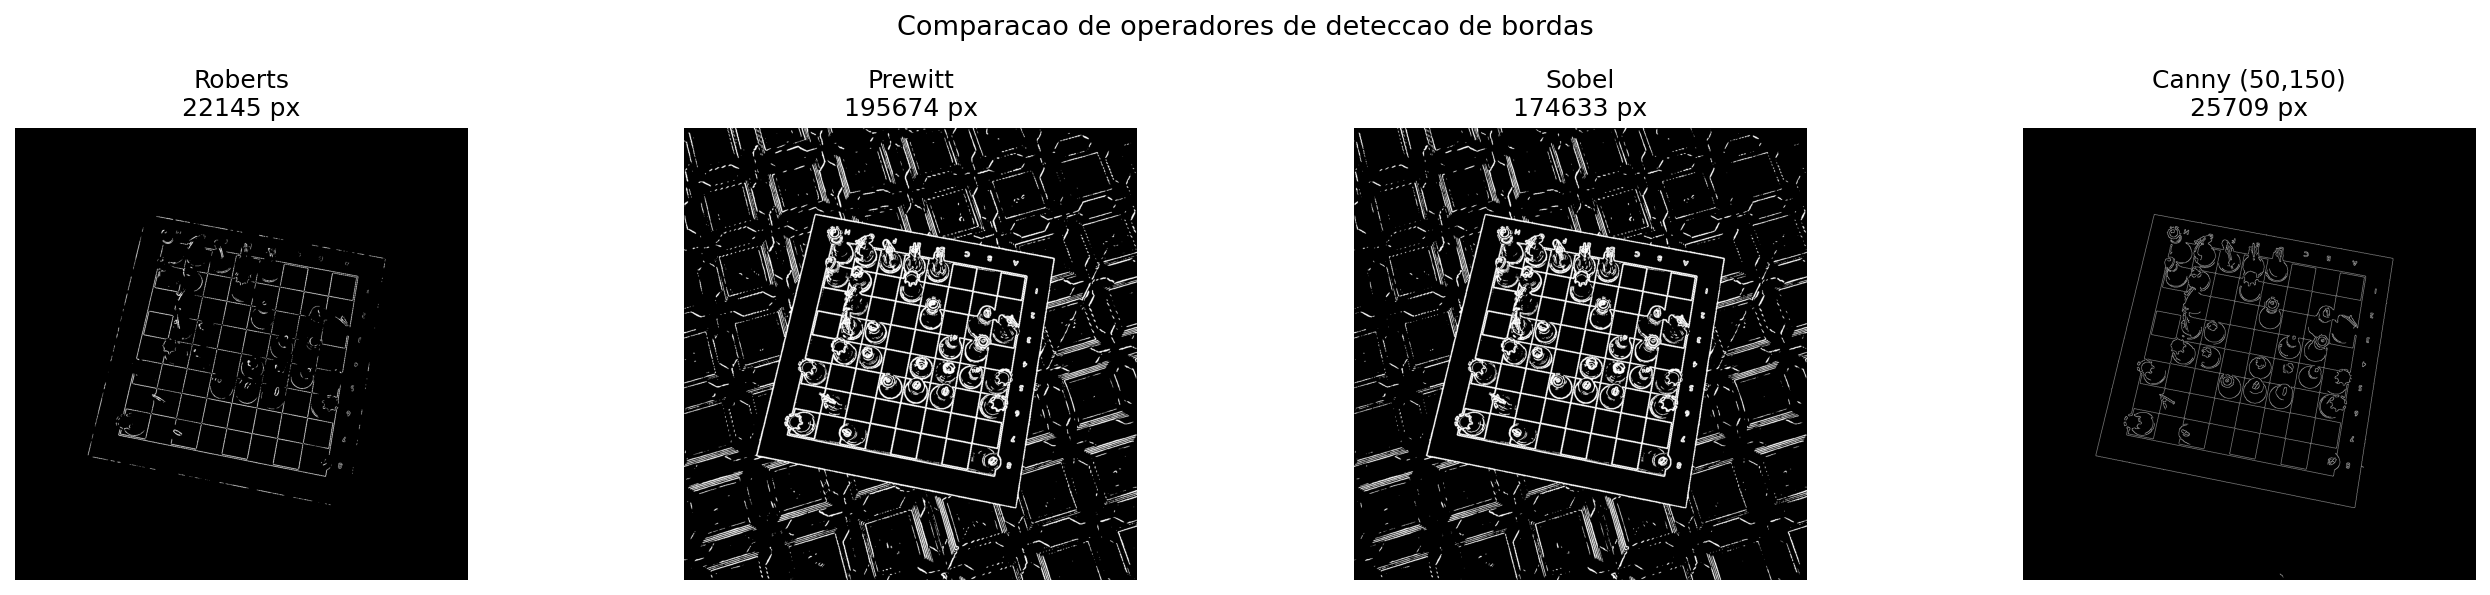
\includegraphics[width=0.85\textwidth]{../../intro/images/04b_edge_operators_comparison.png}
  \caption{Comparação entre operadores de borda Roberts, Prewitt, Sobel e Canny.}
\end{figure}

Operações morfológicas (erosão e dilatação $3\times3$, abertura e fechamento
$5\times5$) são aplicadas sobre a imagem binária de bordas para remover ruído pontual e
conectar segmentos de borda próximos.

\subsection{Detecção de linhas --- Transformada de Hough}

A Transformada de Hough converte o problema de detectar linhas no espaço da imagem em
detectar picos no espaço paramétrico $(\rho, \theta)$: cada pixel de borda vota em todas
as curvas $\rho = x\cos\theta + y\sin\theta$ compatíveis, e picos do acumulador acima de
um limiar indicam linhas reais (\texttt{cv2.HoughLines}, $\rho=1\,\text{px}$,
$\theta=\pi/180\,\text{rad}$, \texttt{threshold} entre 80 e 100).

As linhas detectadas são classificadas em horizontais ($\theta \approx \pi/2$) e
verticais ($\theta \approx 0$). Um algoritmo de janela deslizante seleciona, em cada
direção, as 9 linhas mais igualmente espaçadas, correspondendo às 9 linhas de grade do
tabuleiro $8\times8$. O dataset inclui uma borda de madeira ao redor do grid de jogo; a
última linha horizontal detectada corresponde a essa borda e é descartada --- os cantos
do tabuleiro de jogo são calculados usando a penúltima linha como borda inferior real.

\begin{figure}[H]
  \centering
  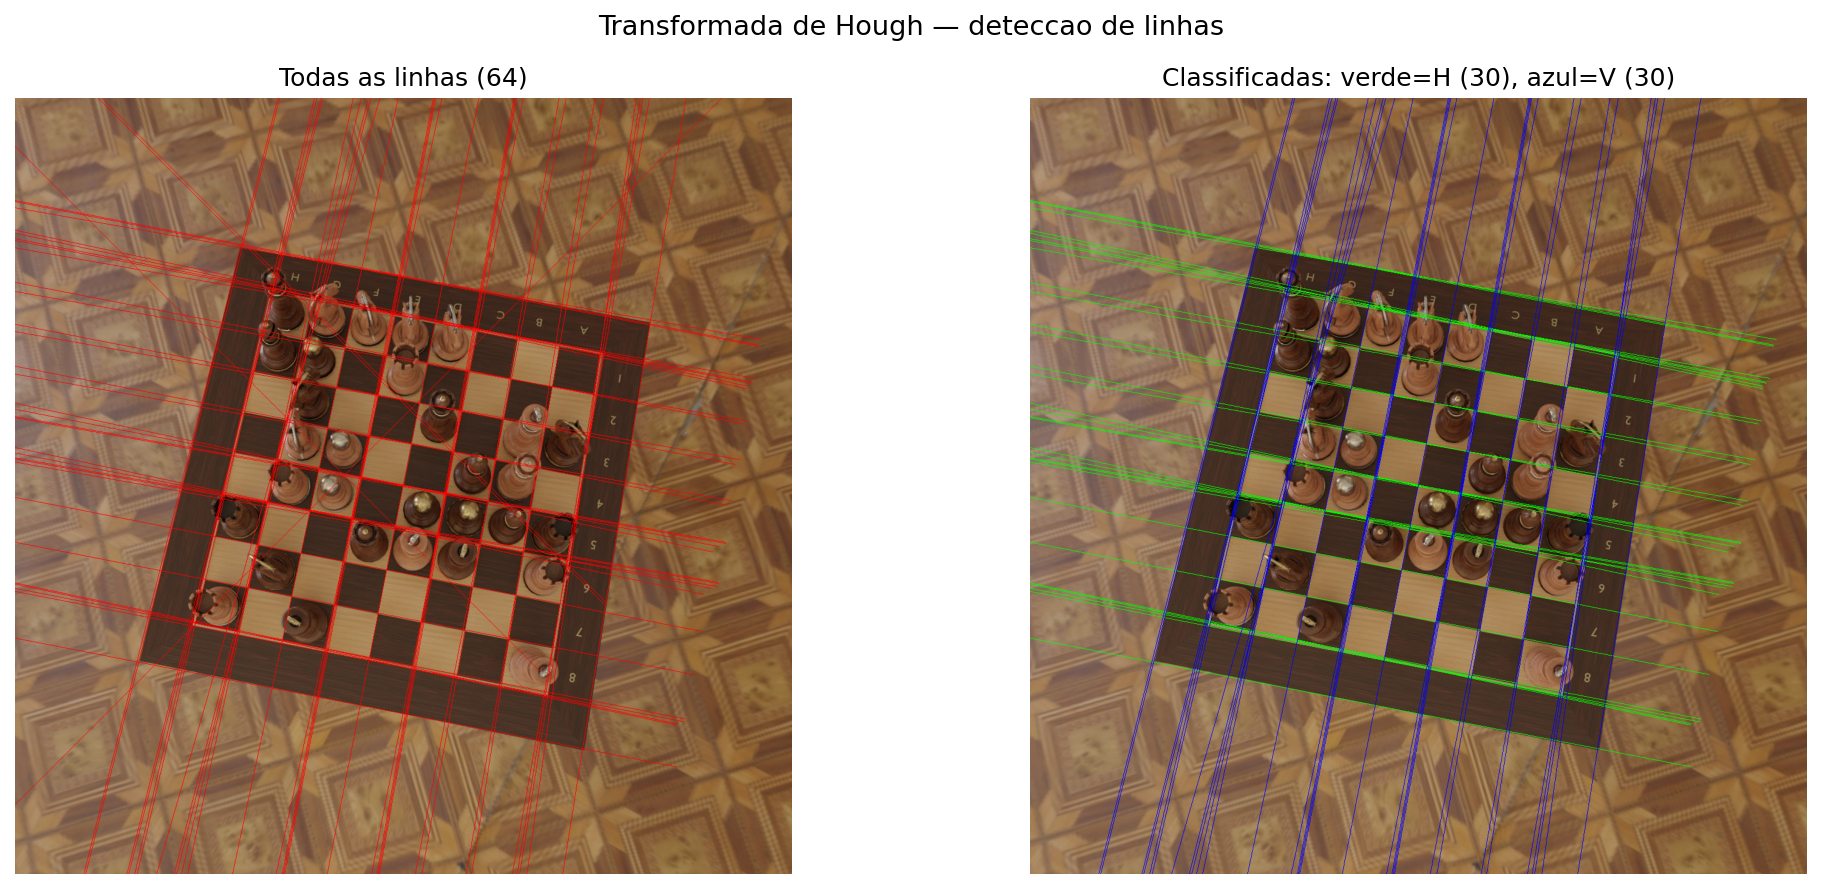
\includegraphics[width=0.7\textwidth]{../../intro/images/05_hough_lines.png}
  \caption{Linhas horizontais (verde) e verticais (azul) detectadas via Hough.}
\end{figure}

\subsection{Correção de perspectiva --- homografia}

Uma homografia (matriz projetiva $3\times3$) mapeia os 4 cantos detectados do tabuleiro
para os cantos de um quadrado de destino de $480\times480$ pixels
(\texttt{cv2.findHomography} + \texttt{cv2.warpPerspective}), produzindo uma vista de
cima onde cada uma das 64 casas ocupa exatamente $60\times60$ pixels. A função de
detecção de cantos (\texttt{detect\_board\_corners\_combined}) executa toda a pipeline
de bordas e Hough sem usar anotações; em caso de falha, os cantos anotados no JSON do
dataset são usados como \textit{fallback}.

Como a câmera fotografa o tabuleiro de ângulos variados, a orientação do mapa de
ocupação resultante pode estar rotacionada em $0\degree$, $90\degree$, $180\degree$ ou
$270\degree$ em relação ao referencial padrão. Quando o \textit{ground truth} está
disponível, a rotação correta é escolhida por busca exaustiva entre as 4 opções
(\texttt{best\_rotation\_vs\_gt}); no cenário totalmente automático, a orientação é
estimada a partir da densidade de bordas por linha/coluna
(\texttt{detect\_board\_rotation}) --- ver discussão da ambiguidade de $180\degree$ na
Seção~\ref{sec:fen-jogadas}.

\begin{figure}[H]
  \centering
  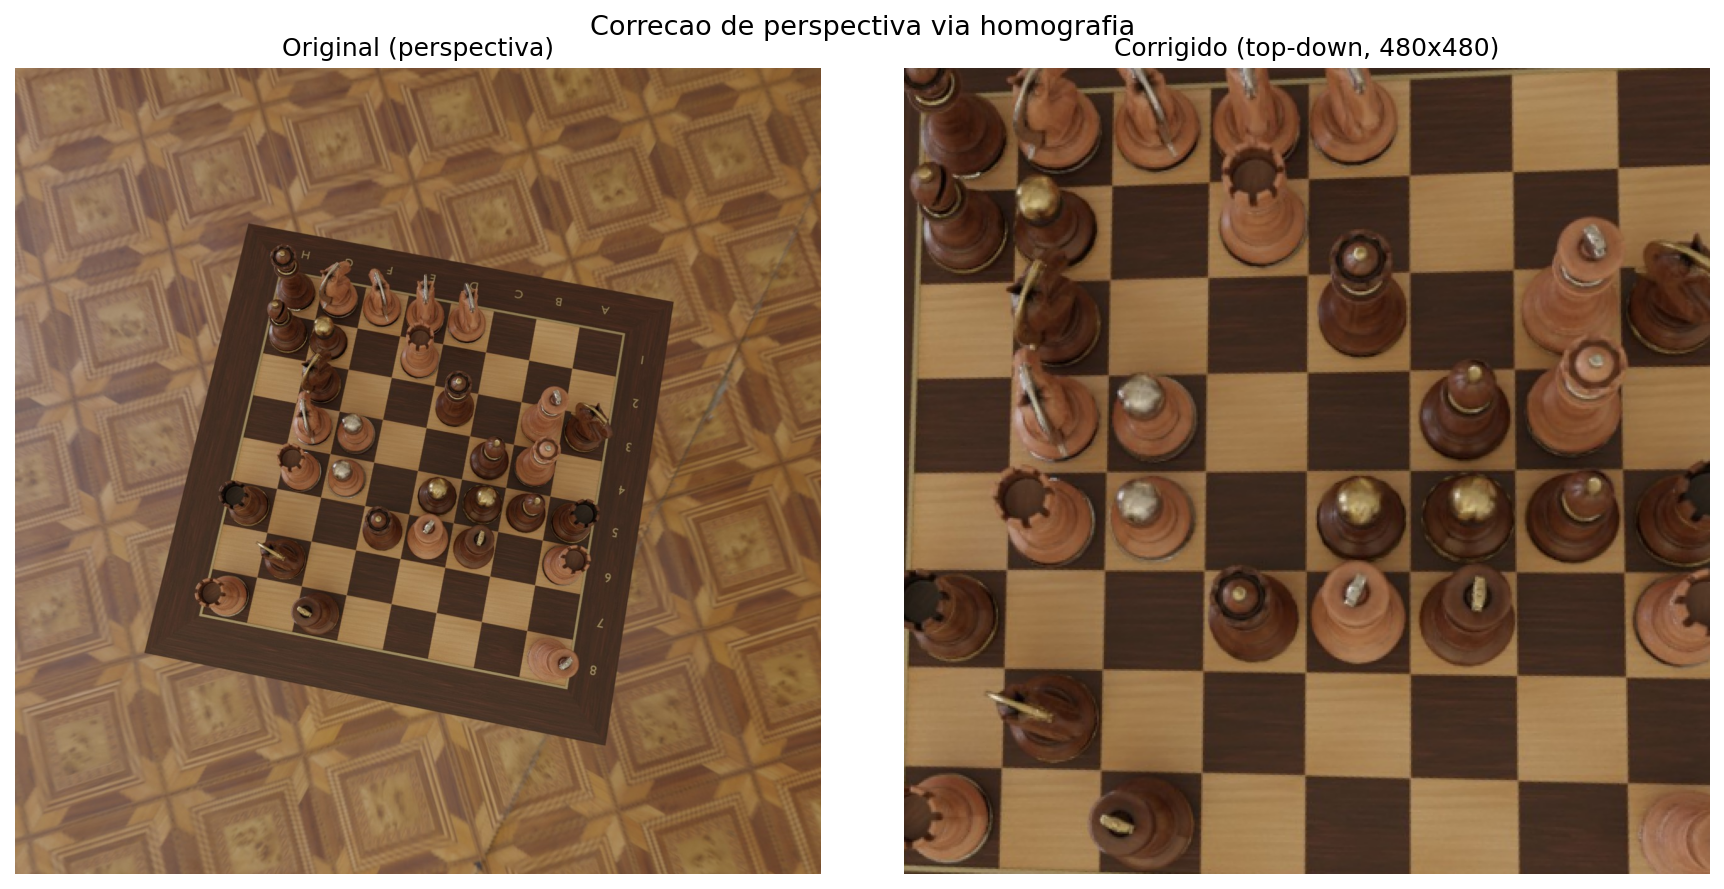
\includegraphics[width=0.6\textwidth]{../../intro/images/07_perspective_correction.png}
  \caption{Correção de perspectiva: da foto em ângulo à vista de cima $480\times480$.}
\end{figure}

\subsection{Segmentação $8\times8$}

Com o tabuleiro retificado, a divisão em 64 casas é um fatiamento uniforme:
$\text{cell}_{r,c} = \text{warped}[r{\cdot}60:(r{+}1){\cdot}60,\; c{\cdot}60:(c{+}1){\cdot}60]$,
produzindo recortes de $60\times60$ pixels indexados de A1 a H8.

\begin{figure}[H]
  \centering
  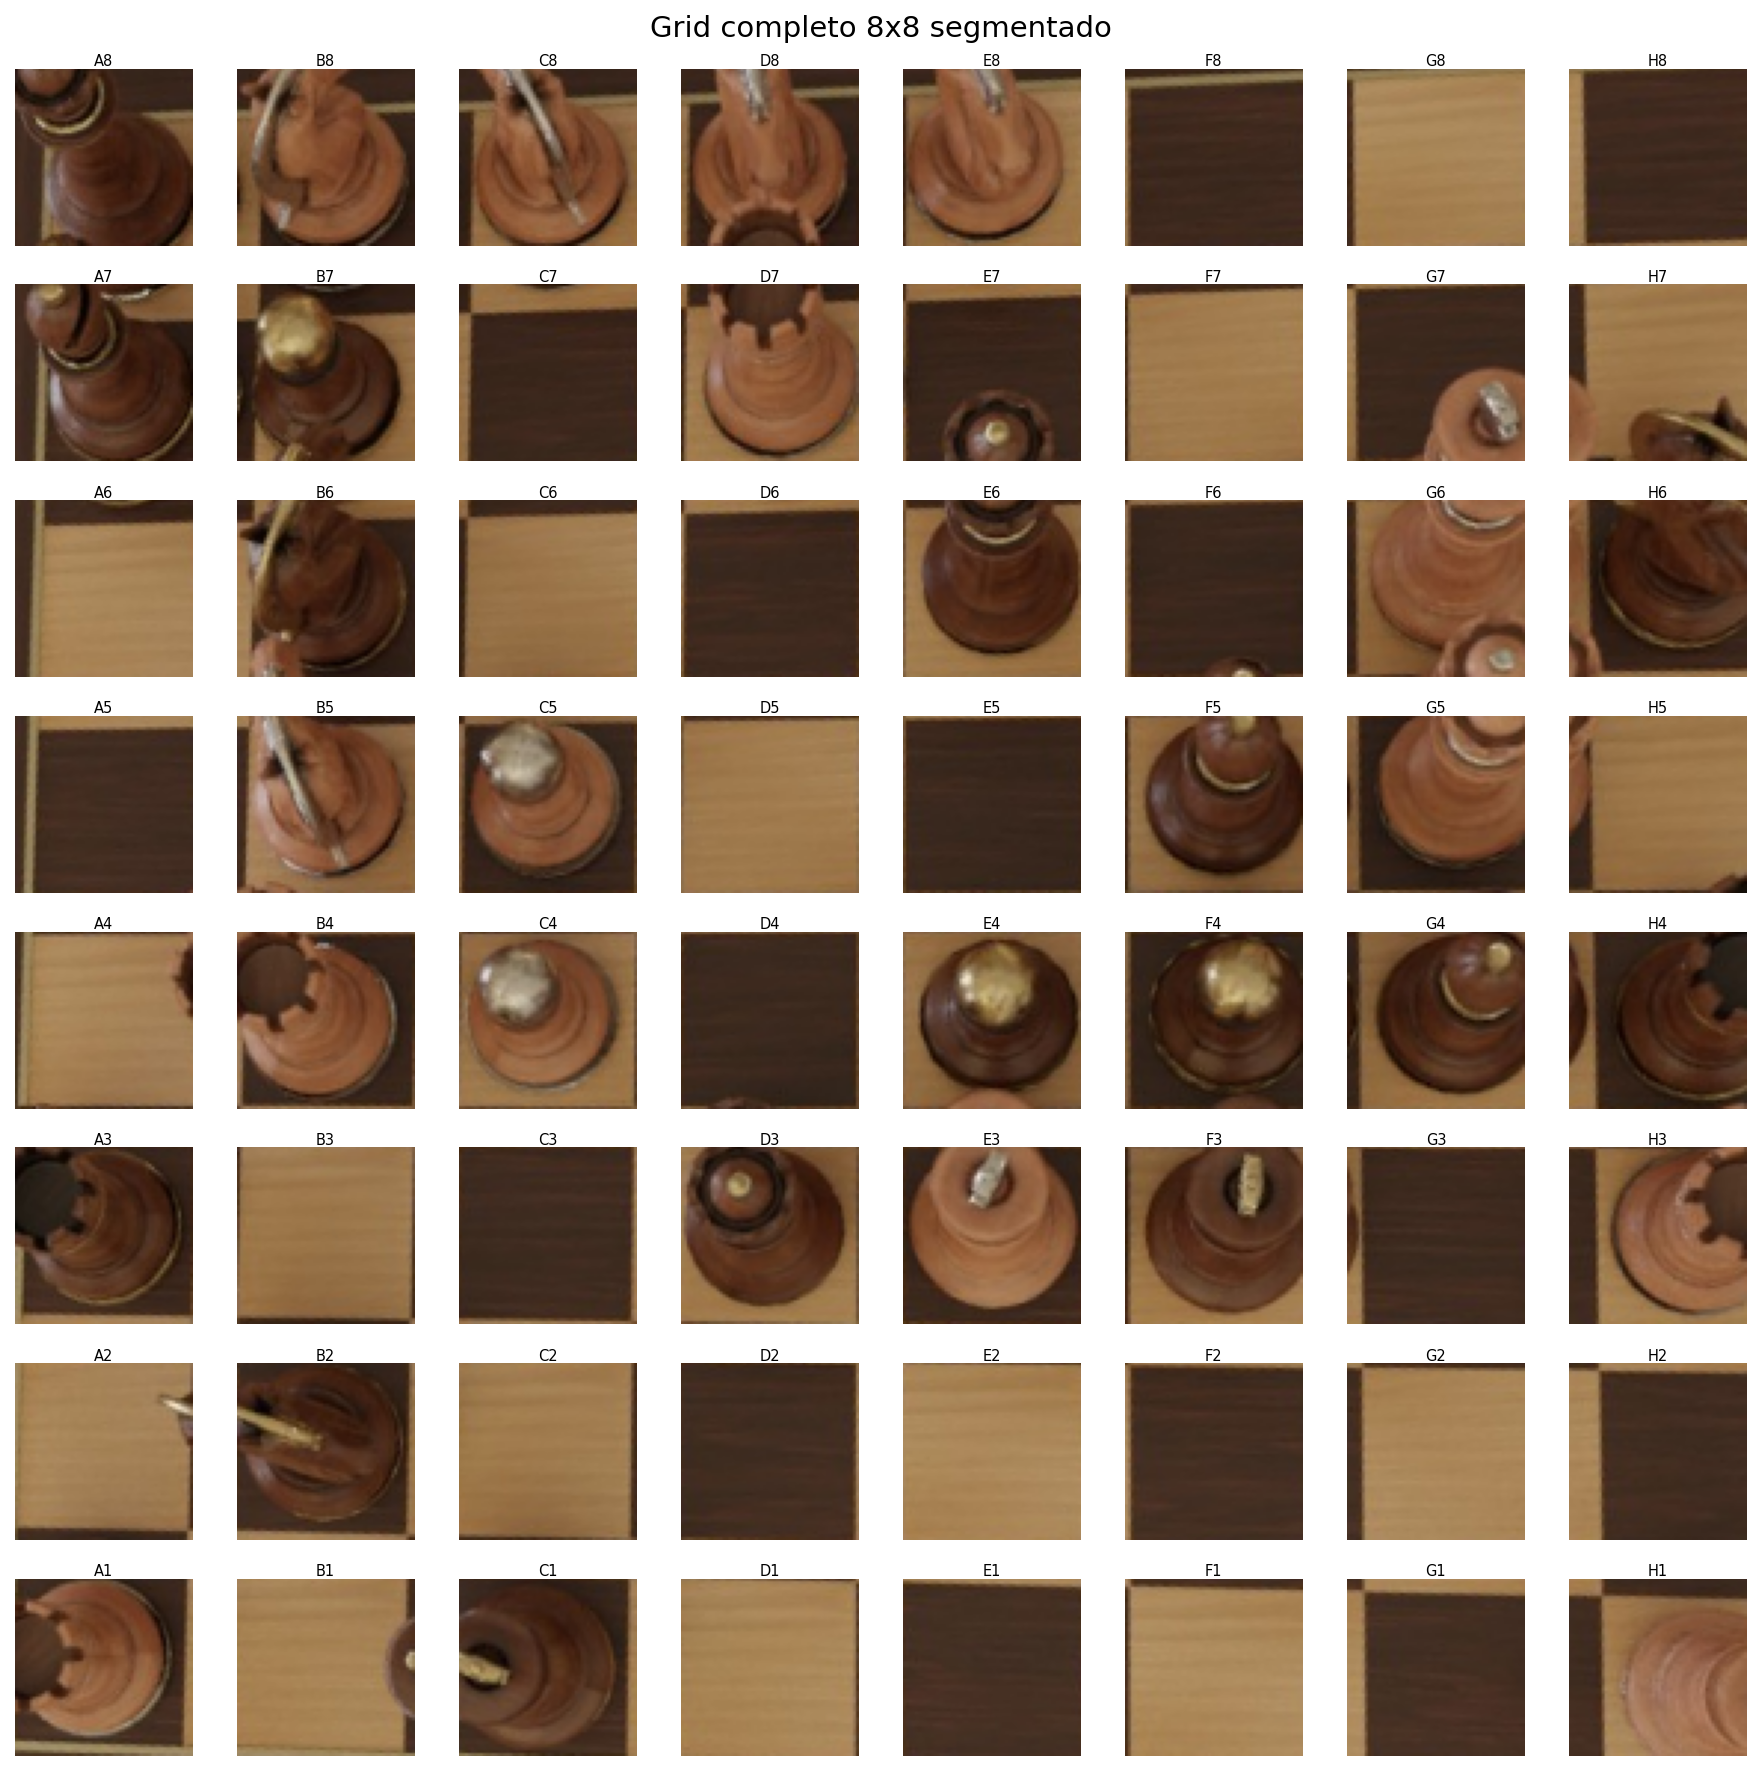
\includegraphics[width=0.55\textwidth]{../../intro/images/08_full_grid.png}
  \caption{Segmentação do tabuleiro retificado em 64 casas individuais.}
\end{figure}

\subsection{Detecção de ocupação}

Para cada casa, quatro descritores clássicos são extraídos e combinados por votação:

\begin{table}[H]
\centering
\caption{Características e limiares do classificador de ocupação por votação.}
\begin{tabular}{@{}llll@{}}
\toprule
Característica & Cálculo & Limiar & Lógica \\
\midrule
Desvio-padrão de intensidade & \texttt{np.std(cell)} & 18 & peças criam variação de brilho \\
Densidade de bordas & \texttt{mean(canny > 0)} & 0,04 & peças geram bordas internas \\
Variância do Laplaciano & \texttt{Laplacian(cell).var()} & 80 & indica textura (peça $\ne$ madeira lisa) \\
Diferença centro-borda & \texttt{mean(centro) - mean(borda)} & 12 & peça ocupa o centro da casa \\
\bottomrule
\end{tabular}
\end{table}

A casa é considerada ocupada quando pelo menos 2 das 4 características ultrapassam seu
limiar (\textit{votos} $\geq 2$). Com material uniforme (madeira sobre madeira), nenhuma
característica isolada é confiável o suficiente; a combinação por maioria simples reduz
falsos positivos e negativos em relação a qualquer característica isolada.

\begin{figure}[H]
  \centering
  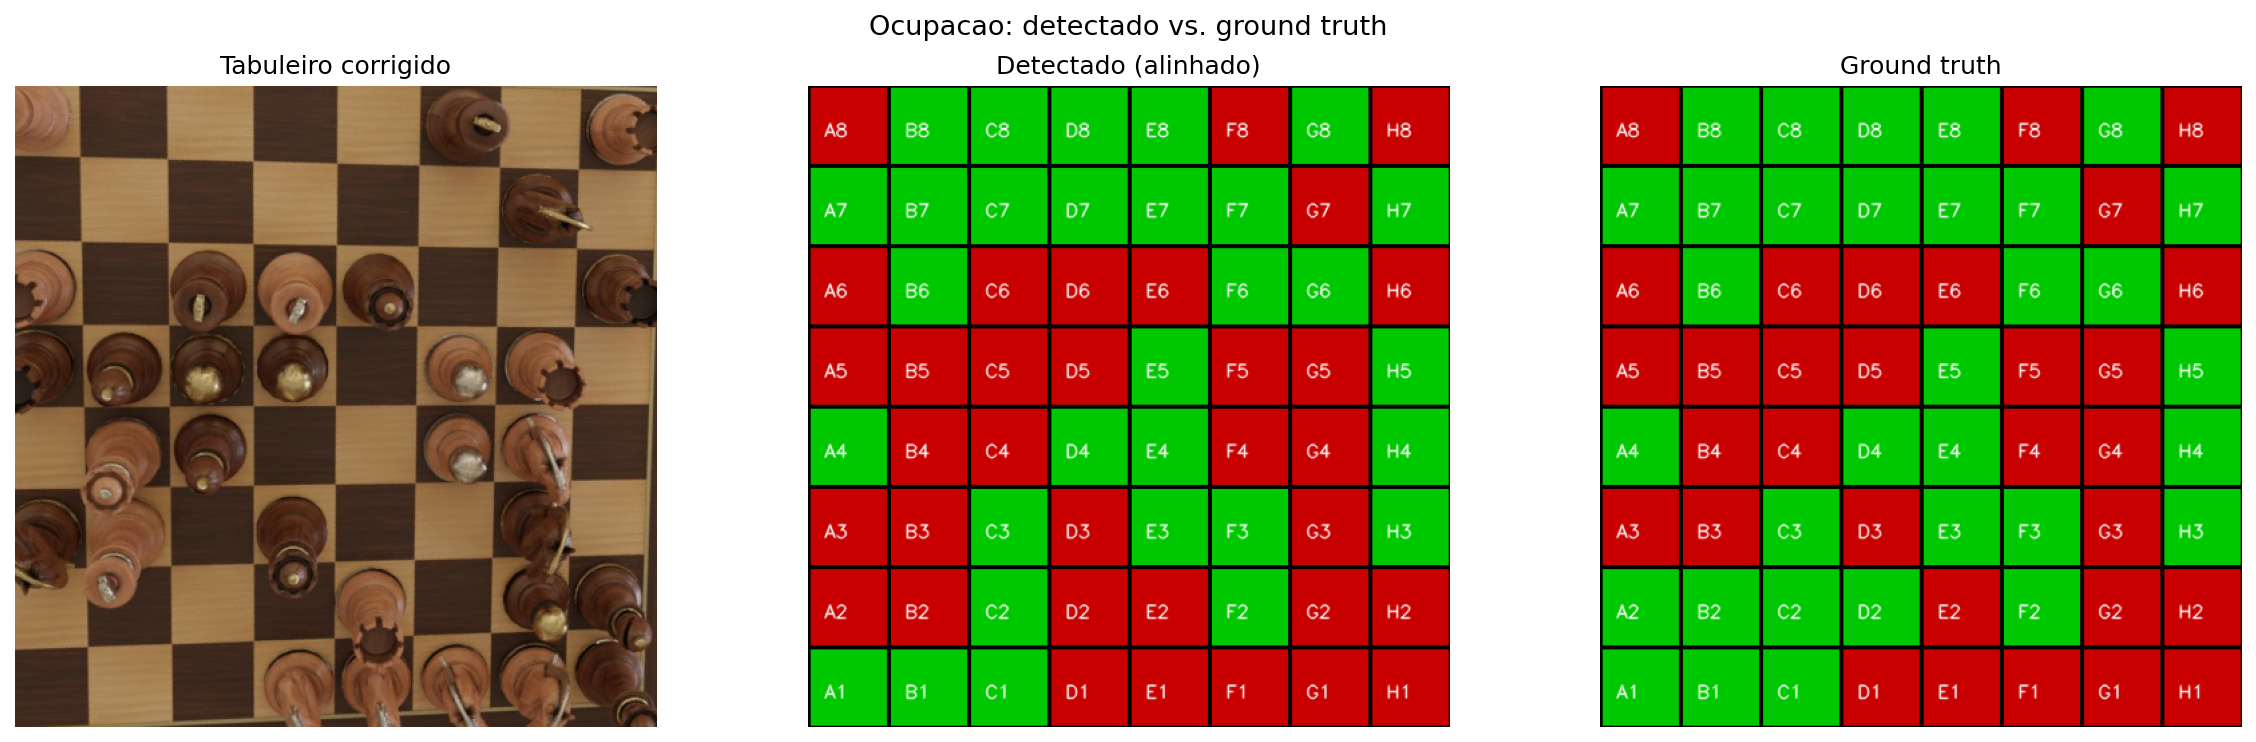
\includegraphics[width=0.7\textwidth]{../../intro/images/10_occupancy_comparison.png}
  \caption{Ocupação detectada (vermelho = ocupada, verde = vazia) comparada ao gabarito.}
\end{figure}

\subsection{Classificação de cor}

A cor de cada peça (clara ou escura) é decidida pelo canal V (\textit{value}, brilho) do
espaço HSV: \texttt{mean\_v = np.mean(hsv[:,:,2])}; peças com \texttt{mean\_v} acima de
um limiar fixo são classificadas como claras, abaixo como escuras. Peças claras
(\textit{boxwood}) têm maior brilho médio que peças escuras (\textit{ebony}), o que
torna essa distinção robusta na maior parte das imagens --- exceto em casos de sombra
projetada ou peça escura sobre casa escura, onde o limiar fixo falha (ver
Seção~\ref{sec:resultados}).

\begin{figure}[H]
  \centering
  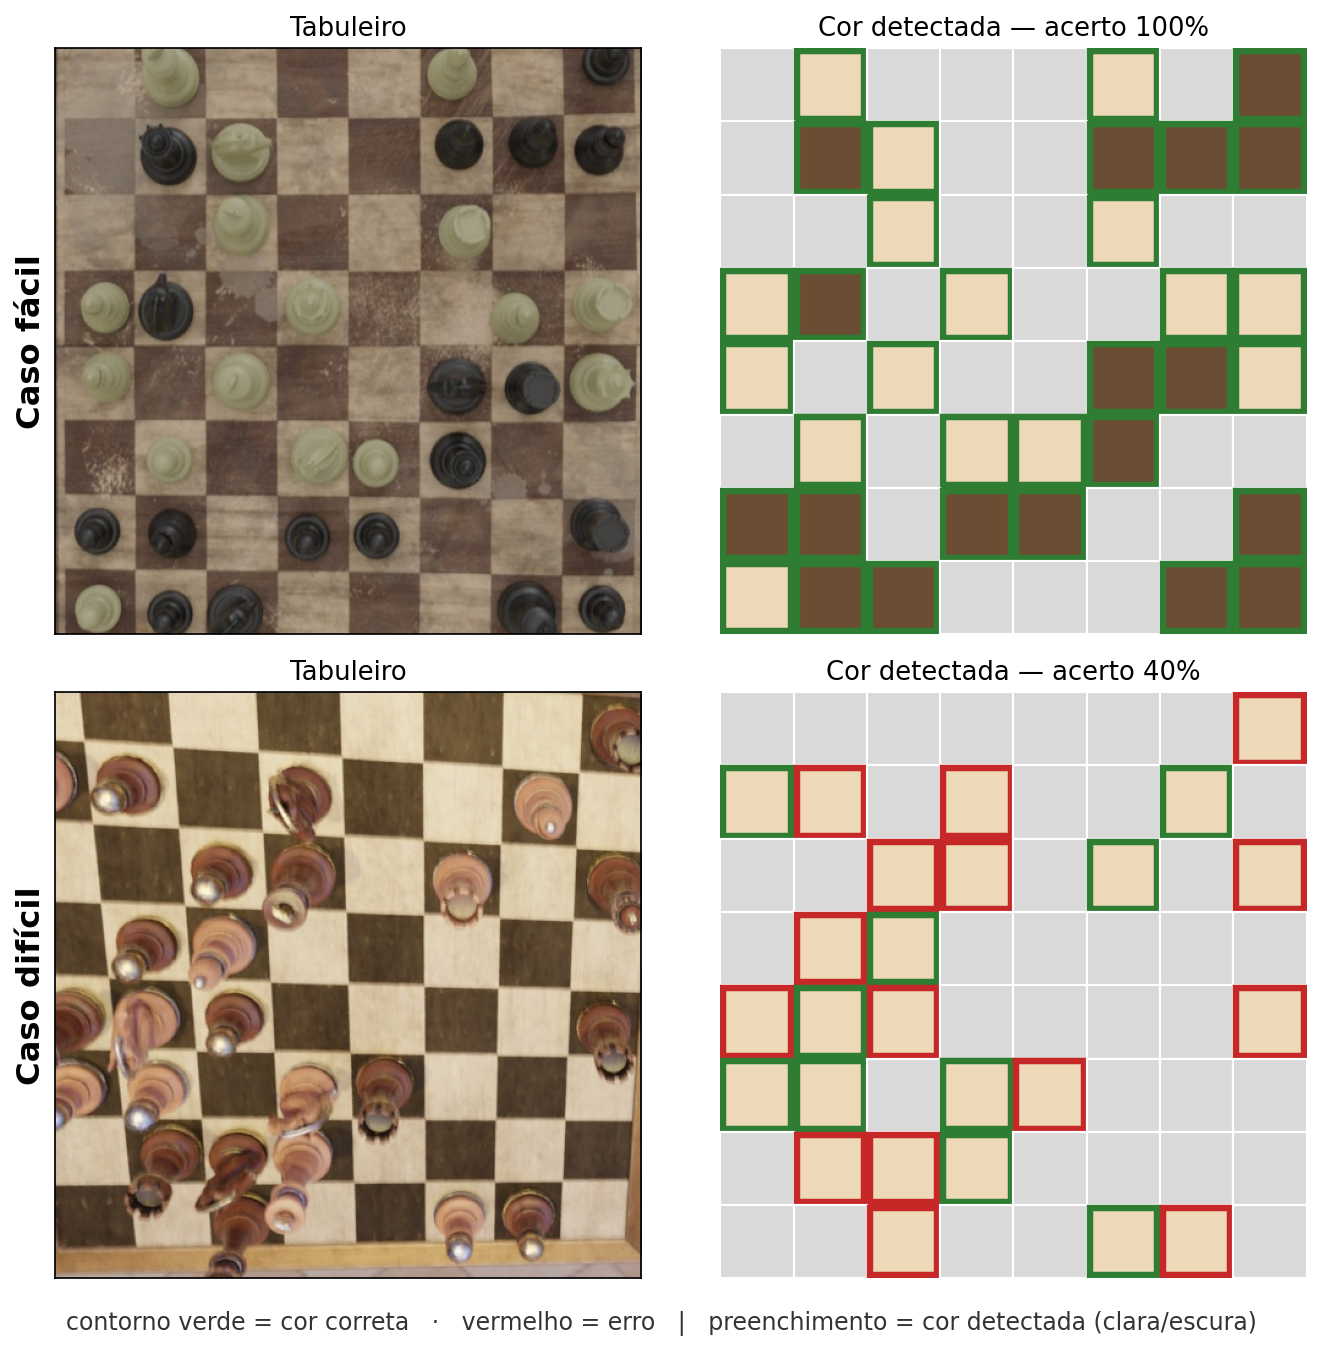
\includegraphics[width=0.6\textwidth]{../../andamento/images/11b_color_cases.png}
  \caption{Casos fáceis e difíceis de classificação de cor por limiar HSV.}
\end{figure}
